% Created by tikzDevice version 0.12.3.1 on 2022-07-12 09:05:21
% !TEX encoding = UTF-8 Unicode
\documentclass{standalone}
\usepackage[table]{xcolor}
\usepackage{tikz}
\usepackage{fontspec}
\usepackage[abspath]{currfile}
\usepackage{booktabs}
\setmainfont[
Path={C:/Users/pgalvez/OneDrive - ine.gob.gt/Documentos/GitHub/CompendioGenero2023/Codigo/Fuentes/},,
BoldFont = OpenSans-CondBold.ttf ,
ItalicFont = OpenSans-CondLightItalic.ttf ,
BoldItalicFont = OpenSans-CondLightItalic.ttf
]{OpenSans-CondLight.ttf}
\newfontfamily\Bold{Open Sans Condensed Bold}
\newfontfamily\Sans{Open Sans}
\newfontfamily\SansBold{Open Sans Bold}
\newfontfamily\Italic{Open Sans Condensed Light Italic}
\newfontfamily\Logos{Latin Modern Roman}
\newfontfamily\Cinzel{Open Sans}

\usetikzlibrary{calc}
\usetikzlibrary{positioning}
\begin{document}
	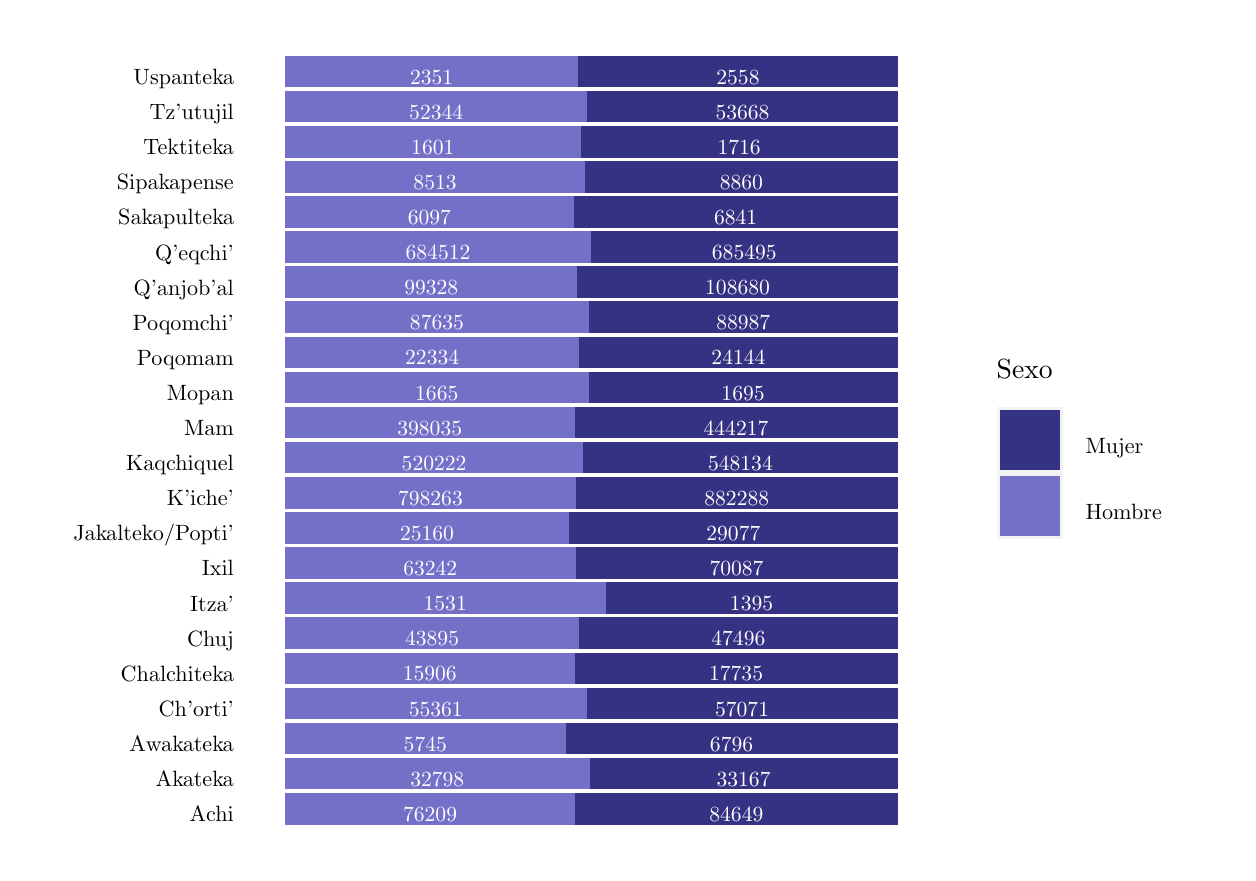
\begin{tikzpicture}[x=1pt,y=1pt, scale = 1.5]
		% Created by tikzDevice version 0.12.4 on 2023-04-20 09:23:04
% !TEX encoding = UTF-8 Unicode
\definecolor{fillColor}{RGB}{255,255,255}
\path[use as bounding box,fill=fillColor,fill opacity=0.00] (0,0) rectangle (289.08,198.74);
\begin{scope}
\path[clip] (  0.00,  0.00) rectangle (289.08,198.74);
\definecolor{drawColor}{RGB}{255,255,255}
\definecolor{fillColor}{RGB}{255,255,255}

\path[draw=drawColor,line width= 0.6pt,line join=round,line cap=round,fill=fillColor] (  0.00,  0.00) rectangle (289.08,198.74);
\end{scope}
\begin{scope}
\path[clip] (  0.00,  0.00) rectangle (289.08,198.74);
\definecolor{fillColor}{RGB}{54,50,131}

\path[fill=fillColor] (131.90,  6.77) rectangle (209.56, 14.38);

\path[fill=fillColor] (135.36, 15.23) rectangle (209.56, 22.84);

\path[fill=fillColor] (129.59, 23.68) rectangle (209.56, 31.29);

\path[fill=fillColor] (134.65, 32.14) rectangle (209.56, 39.75);

\path[fill=fillColor] (131.76, 40.60) rectangle (209.56, 48.21);

\path[fill=fillColor] (132.86, 49.05) rectangle (209.56, 56.66);

\path[fill=fillColor] (139.20, 57.51) rectangle (209.56, 65.12);

\path[fill=fillColor] (131.98, 65.97) rectangle (209.56, 73.58);

\path[fill=fillColor] (130.44, 74.42) rectangle (209.56, 82.03);

\path[fill=fillColor] (132.08, 82.88) rectangle (209.56, 90.49);

\path[fill=fillColor] (133.84, 91.34) rectangle (209.56, 98.95);

\path[fill=fillColor] (131.73, 99.79) rectangle (209.56,107.41);

\path[fill=fillColor] (135.11,108.25) rectangle (209.56,115.86);

\path[fill=fillColor] (132.90,116.71) rectangle (209.56,124.32);

\path[fill=fillColor] (135.21,125.16) rectangle (209.56,132.78);

\path[fill=fillColor] (132.45,133.62) rectangle (209.56,141.23);

\path[fill=fillColor] (135.72,142.08) rectangle (209.56,149.69);

\path[fill=fillColor] (131.53,150.54) rectangle (209.56,158.15);

\path[fill=fillColor] (134.30,158.99) rectangle (209.56,166.60);

\path[fill=fillColor] (133.21,167.45) rectangle (209.56,175.06);

\path[fill=fillColor] (134.85,175.91) rectangle (209.56,183.52);

\path[fill=fillColor] (132.66,184.36) rectangle (209.56,191.97);
\definecolor{fillColor}{RGB}{116,112,200}

\path[fill=fillColor] ( 61.98,  6.77) rectangle (131.90, 14.38);

\path[fill=fillColor] ( 61.98, 15.23) rectangle (135.36, 22.84);

\path[fill=fillColor] ( 61.98, 23.68) rectangle (129.59, 31.29);

\path[fill=fillColor] ( 61.98, 32.14) rectangle (134.65, 39.75);

\path[fill=fillColor] ( 61.98, 40.60) rectangle (131.76, 48.21);

\path[fill=fillColor] ( 61.98, 49.05) rectangle (132.86, 56.66);

\path[fill=fillColor] ( 61.98, 57.51) rectangle (139.20, 65.12);

\path[fill=fillColor] ( 61.98, 65.97) rectangle (131.98, 73.58);

\path[fill=fillColor] ( 61.98, 74.42) rectangle (130.44, 82.03);

\path[fill=fillColor] ( 61.98, 82.88) rectangle (132.08, 90.49);

\path[fill=fillColor] ( 61.98, 91.34) rectangle (133.84, 98.95);

\path[fill=fillColor] ( 61.98, 99.79) rectangle (131.73,107.41);

\path[fill=fillColor] ( 61.98,108.25) rectangle (135.11,115.86);

\path[fill=fillColor] ( 61.98,116.71) rectangle (132.90,124.32);

\path[fill=fillColor] ( 61.98,125.16) rectangle (135.21,132.78);

\path[fill=fillColor] ( 61.98,133.62) rectangle (132.45,141.23);

\path[fill=fillColor] ( 61.98,142.08) rectangle (135.72,149.69);

\path[fill=fillColor] ( 61.98,150.54) rectangle (131.53,158.15);

\path[fill=fillColor] ( 61.98,158.99) rectangle (134.30,166.60);

\path[fill=fillColor] ( 61.98,167.45) rectangle (133.21,175.06);

\path[fill=fillColor] ( 61.98,175.91) rectangle (134.85,183.52);

\path[fill=fillColor] ( 61.98,184.36) rectangle (132.66,191.97);
\definecolor{drawColor}{RGB}{255,255,255}

\node[text=drawColor,anchor=base,inner sep=0pt, outer sep=0pt, scale=  0.78] at (170.73,  7.54) {84649};

\node[text=drawColor,anchor=base,inner sep=0pt, outer sep=0pt, scale=  0.78] at (172.46, 16.00) {33167};

\node[text=drawColor,anchor=base,inner sep=0pt, outer sep=0pt, scale=  0.78] at (169.57, 24.45) {6796};

\node[text=drawColor,anchor=base,inner sep=0pt, outer sep=0pt, scale=  0.78] at (172.10, 32.91) {57071};

\node[text=drawColor,anchor=base,inner sep=0pt, outer sep=0pt, scale=  0.78] at (170.66, 41.37) {17735};

\node[text=drawColor,anchor=base,inner sep=0pt, outer sep=0pt, scale=  0.78] at (171.21, 49.83) {47496};

\node[text=drawColor,anchor=base,inner sep=0pt, outer sep=0pt, scale=  0.78] at (174.38, 58.28) {1395};

\node[text=drawColor,anchor=base,inner sep=0pt, outer sep=0pt, scale=  0.78] at (170.77, 66.74) {70087};

\node[text=drawColor,anchor=base,inner sep=0pt, outer sep=0pt, scale=  0.78] at (170.00, 75.20) {29077};

\node[text=drawColor,anchor=base,inner sep=0pt, outer sep=0pt, scale=  0.78] at (170.82, 83.65) {882288};

\node[text=drawColor,anchor=base,inner sep=0pt, outer sep=0pt, scale=  0.78] at (171.70, 92.11) {548134};

\node[text=drawColor,anchor=base,inner sep=0pt, outer sep=0pt, scale=  0.78] at (170.64,100.57) {444217};

\node[text=drawColor,anchor=base,inner sep=0pt, outer sep=0pt, scale=  0.78] at (172.34,109.02) {1695};

\node[text=drawColor,anchor=base,inner sep=0pt, outer sep=0pt, scale=  0.78] at (171.23,117.48) {24144};

\node[text=drawColor,anchor=base,inner sep=0pt, outer sep=0pt, scale=  0.78] at (172.38,125.94) {88987};

\node[text=drawColor,anchor=base,inner sep=0pt, outer sep=0pt, scale=  0.78] at (171.01,134.39) {108680};

\node[text=drawColor,anchor=base,inner sep=0pt, outer sep=0pt, scale=  0.78] at (172.64,142.85) {685495};

\node[text=drawColor,anchor=base,inner sep=0pt, outer sep=0pt, scale=  0.78] at (170.54,151.31) {6841};

\node[text=drawColor,anchor=base,inner sep=0pt, outer sep=0pt, scale=  0.78] at (171.93,159.76) {8860};

\node[text=drawColor,anchor=base,inner sep=0pt, outer sep=0pt, scale=  0.78] at (171.39,168.22) {1716};

\node[text=drawColor,anchor=base,inner sep=0pt, outer sep=0pt, scale=  0.78] at (172.20,176.68) {53668};

\node[text=drawColor,anchor=base,inner sep=0pt, outer sep=0pt, scale=  0.78] at (171.11,185.14) {2558};

\node[text=drawColor,anchor=base,inner sep=0pt, outer sep=0pt, scale=  0.78] at ( 96.94,  7.54) {76209};

\node[text=drawColor,anchor=base,inner sep=0pt, outer sep=0pt, scale=  0.78] at ( 98.67, 16.00) {32798};

\node[text=drawColor,anchor=base,inner sep=0pt, outer sep=0pt, scale=  0.78] at ( 95.79, 24.45) {5745};

\node[text=drawColor,anchor=base,inner sep=0pt, outer sep=0pt, scale=  0.78] at ( 98.32, 32.91) {55361};

\node[text=drawColor,anchor=base,inner sep=0pt, outer sep=0pt, scale=  0.78] at ( 96.87, 41.37) {15906};

\node[text=drawColor,anchor=base,inner sep=0pt, outer sep=0pt, scale=  0.78] at ( 97.42, 49.83) {43895};

\node[text=drawColor,anchor=base,inner sep=0pt, outer sep=0pt, scale=  0.78] at (100.59, 58.28) {1531};

\node[text=drawColor,anchor=base,inner sep=0pt, outer sep=0pt, scale=  0.78] at ( 96.98, 66.74) {63242};

\node[text=drawColor,anchor=base,inner sep=0pt, outer sep=0pt, scale=  0.78] at ( 96.21, 75.20) {25160};

\node[text=drawColor,anchor=base,inner sep=0pt, outer sep=0pt, scale=  0.78] at ( 97.03, 83.65) {798263};

\node[text=drawColor,anchor=base,inner sep=0pt, outer sep=0pt, scale=  0.78] at ( 97.91, 92.11) {520222};

\node[text=drawColor,anchor=base,inner sep=0pt, outer sep=0pt, scale=  0.78] at ( 96.85,100.57) {398035};

\node[text=drawColor,anchor=base,inner sep=0pt, outer sep=0pt, scale=  0.78] at ( 98.55,109.02) {1665};

\node[text=drawColor,anchor=base,inner sep=0pt, outer sep=0pt, scale=  0.78] at ( 97.44,117.48) {22334};

\node[text=drawColor,anchor=base,inner sep=0pt, outer sep=0pt, scale=  0.78] at ( 98.60,125.94) {87635};

\node[text=drawColor,anchor=base,inner sep=0pt, outer sep=0pt, scale=  0.78] at ( 97.22,134.39) {99328};

\node[text=drawColor,anchor=base,inner sep=0pt, outer sep=0pt, scale=  0.78] at ( 98.85,142.85) {684512};

\node[text=drawColor,anchor=base,inner sep=0pt, outer sep=0pt, scale=  0.78] at ( 96.76,151.31) {6097};

\node[text=drawColor,anchor=base,inner sep=0pt, outer sep=0pt, scale=  0.78] at ( 98.14,159.76) {8513};

\node[text=drawColor,anchor=base,inner sep=0pt, outer sep=0pt, scale=  0.78] at ( 97.60,168.22) {1601};

\node[text=drawColor,anchor=base,inner sep=0pt, outer sep=0pt, scale=  0.78] at ( 98.42,176.68) {52344};

\node[text=drawColor,anchor=base,inner sep=0pt, outer sep=0pt, scale=  0.78] at ( 97.32,185.14) {2351};
\end{scope}
\begin{scope}
\path[clip] (  0.00,  0.00) rectangle (289.08,198.74);
\definecolor{drawColor}{RGB}{0,0,0}

\node[text=drawColor,anchor=base east,inner sep=0pt, outer sep=0pt, scale=  0.80] at ( 49.66,  7.45) {Achi};

\node[text=drawColor,anchor=base east,inner sep=0pt, outer sep=0pt, scale=  0.80] at ( 49.66, 15.90) {Akateka};

\node[text=drawColor,anchor=base east,inner sep=0pt, outer sep=0pt, scale=  0.80] at ( 49.66, 24.36) {Awakateka};

\node[text=drawColor,anchor=base east,inner sep=0pt, outer sep=0pt, scale=  0.80] at ( 49.66, 32.82) {Ch'orti'};

\node[text=drawColor,anchor=base east,inner sep=0pt, outer sep=0pt, scale=  0.80] at ( 49.66, 41.27) {Chalchiteka};

\node[text=drawColor,anchor=base east,inner sep=0pt, outer sep=0pt, scale=  0.80] at ( 49.66, 49.73) {Chuj};

\node[text=drawColor,anchor=base east,inner sep=0pt, outer sep=0pt, scale=  0.80] at ( 49.66, 58.19) {Itza'};

\node[text=drawColor,anchor=base east,inner sep=0pt, outer sep=0pt, scale=  0.80] at ( 49.66, 66.65) {Ixil};

\node[text=drawColor,anchor=base east,inner sep=0pt, outer sep=0pt, scale=  0.80] at ( 49.66, 75.10) {Jakalteko/Popti'};

\node[text=drawColor,anchor=base east,inner sep=0pt, outer sep=0pt, scale=  0.80] at ( 49.66, 83.56) {K'iche'};

\node[text=drawColor,anchor=base east,inner sep=0pt, outer sep=0pt, scale=  0.80] at ( 49.66, 92.02) {Kaqchiquel};

\node[text=drawColor,anchor=base east,inner sep=0pt, outer sep=0pt, scale=  0.80] at ( 49.66,100.47) {Mam};

\node[text=drawColor,anchor=base east,inner sep=0pt, outer sep=0pt, scale=  0.80] at ( 49.66,108.93) {Mopan};

\node[text=drawColor,anchor=base east,inner sep=0pt, outer sep=0pt, scale=  0.80] at ( 49.66,117.39) {Poqomam};

\node[text=drawColor,anchor=base east,inner sep=0pt, outer sep=0pt, scale=  0.80] at ( 49.66,125.84) {Poqomchi'};

\node[text=drawColor,anchor=base east,inner sep=0pt, outer sep=0pt, scale=  0.80] at ( 49.66,134.30) {Q'anjob'al};

\node[text=drawColor,anchor=base east,inner sep=0pt, outer sep=0pt, scale=  0.80] at ( 49.66,142.76) {Q'eqchi'};

\node[text=drawColor,anchor=base east,inner sep=0pt, outer sep=0pt, scale=  0.80] at ( 49.66,151.21) {Sakapulteka};

\node[text=drawColor,anchor=base east,inner sep=0pt, outer sep=0pt, scale=  0.80] at ( 49.66,159.67) {Sipakapense};

\node[text=drawColor,anchor=base east,inner sep=0pt, outer sep=0pt, scale=  0.80] at ( 49.66,168.13) {Tektiteka};

\node[text=drawColor,anchor=base east,inner sep=0pt, outer sep=0pt, scale=  0.80] at ( 49.66,176.58) {Tz'utujil};

\node[text=drawColor,anchor=base east,inner sep=0pt, outer sep=0pt, scale=  0.80] at ( 49.66,185.04) {Uspanteka};
\end{scope}
\begin{scope}
\path[clip] (  0.00,  0.00) rectangle (289.08,198.74);
\definecolor{fillColor}{RGB}{255,255,255}

\path[fill=fillColor] (227.94, 69.99) rectangle (283.58,128.75);
\end{scope}
\begin{scope}
\path[clip] (  0.00,  0.00) rectangle (289.08,198.74);
\definecolor{drawColor}{RGB}{0,0,0}

\node[text=drawColor,anchor=base west,inner sep=0pt, outer sep=0pt, scale=  1.00] at (233.44,114.11) {Sexo};
\end{scope}
\begin{scope}
\path[clip] (  0.00,  0.00) rectangle (289.08,198.74);
\definecolor{fillColor}{gray}{0.95}

\path[fill=fillColor] (233.44, 91.39) rectangle (249.34,107.29);
\end{scope}
\begin{scope}
\path[clip] (  0.00,  0.00) rectangle (289.08,198.74);
\definecolor{fillColor}{RGB}{54,50,131}

\path[fill=fillColor] (234.15, 92.10) rectangle (248.63,106.58);
\end{scope}
\begin{scope}
\path[clip] (  0.00,  0.00) rectangle (289.08,198.74);
\definecolor{fillColor}{gray}{0.95}

\path[fill=fillColor] (233.44, 75.49) rectangle (249.34, 91.39);
\end{scope}
\begin{scope}
\path[clip] (  0.00,  0.00) rectangle (289.08,198.74);
\definecolor{fillColor}{RGB}{116,112,200}

\path[fill=fillColor] (234.15, 76.20) rectangle (248.63, 90.68);
\end{scope}
\begin{scope}
\path[clip] (  0.00,  0.00) rectangle (289.08,198.74);
\definecolor{drawColor}{RGB}{0,0,0}

\node[text=drawColor,anchor=base west,inner sep=0pt, outer sep=0pt, scale=  0.80] at (254.84, 96.21) {Mujer};
\end{scope}
\begin{scope}
\path[clip] (  0.00,  0.00) rectangle (289.08,198.74);
\definecolor{drawColor}{RGB}{0,0,0}

\node[text=drawColor,anchor=base west,inner sep=0pt, outer sep=0pt, scale=  0.80] at (254.84, 80.32) {Hombre};
\end{scope}

	\end{tikzpicture}
\end{document}
